\documentclass{article}
\usepackage[letterpaper]{geometry}
\usepackage{graphicx}
\usepackage{xcolor}
\usepackage{amsmath}

% typesetting
% Margins and typesetting
\setlength{\textwidth}{5.00in}
\setlength{\oddsidemargin}{3.25in}
\addtolength{\oddsidemargin}{-0.5\textwidth}
\addtolength{\topmargin}{-0.55in}
\addtolength{\textheight}{2.00in}
\linespread{1.08}
\pagestyle{myheadings}
\markboth{}{\color{gray}\sffamily Hogg \& Villar / \texttt{MNIST-plus-plus}}
\sloppy\sloppypar\raggedbottom\frenchspacing

\title{\bfseries MNIST-plus-plus: a benchmark for equivariant learning and reasoning tasks}
\author{David W. Hogg \& Soledad Villar}
\date{}

\begin{document}

\maketitle

\begin{abstract}\noindent
    The objective of this paper is to introduce data, code and benchmarks for simple invariant, equivariant and reasoning tasks. We call our package MNIST-plus-plus. It provides four datasets based on simple tranformations of MNIST and Fashion-MNIST.
\end{abstract}

\section{Introduction}

Real-world learning tasks may require to identify objects in arbitrary orientations and make inference depending on contexts. The objective of this work is to provide toy datasets for these tasks. 

\subsection{Fashion-MNIST-plus}
The Fashion-MNIST-plus dataset takes the Fashion-MNIST data and subject it to random rotations and reflections. This is a natural classification task since clothing doesn't really have a preferred orientation.
The 

In natural images text can appear with different shears and orientations. Therefore it is natural to considered a transformed version of MNIST. However, handwritten digits may not be identifiable after rotations or reflections (6s and 9s, 2s and 5s, or even 2s and 6s may look indistinguishable after these transformations). To make the learning problem well-defined our dataset includes contextual information that allows to determine the orientation a

\begin{figure}[tp]
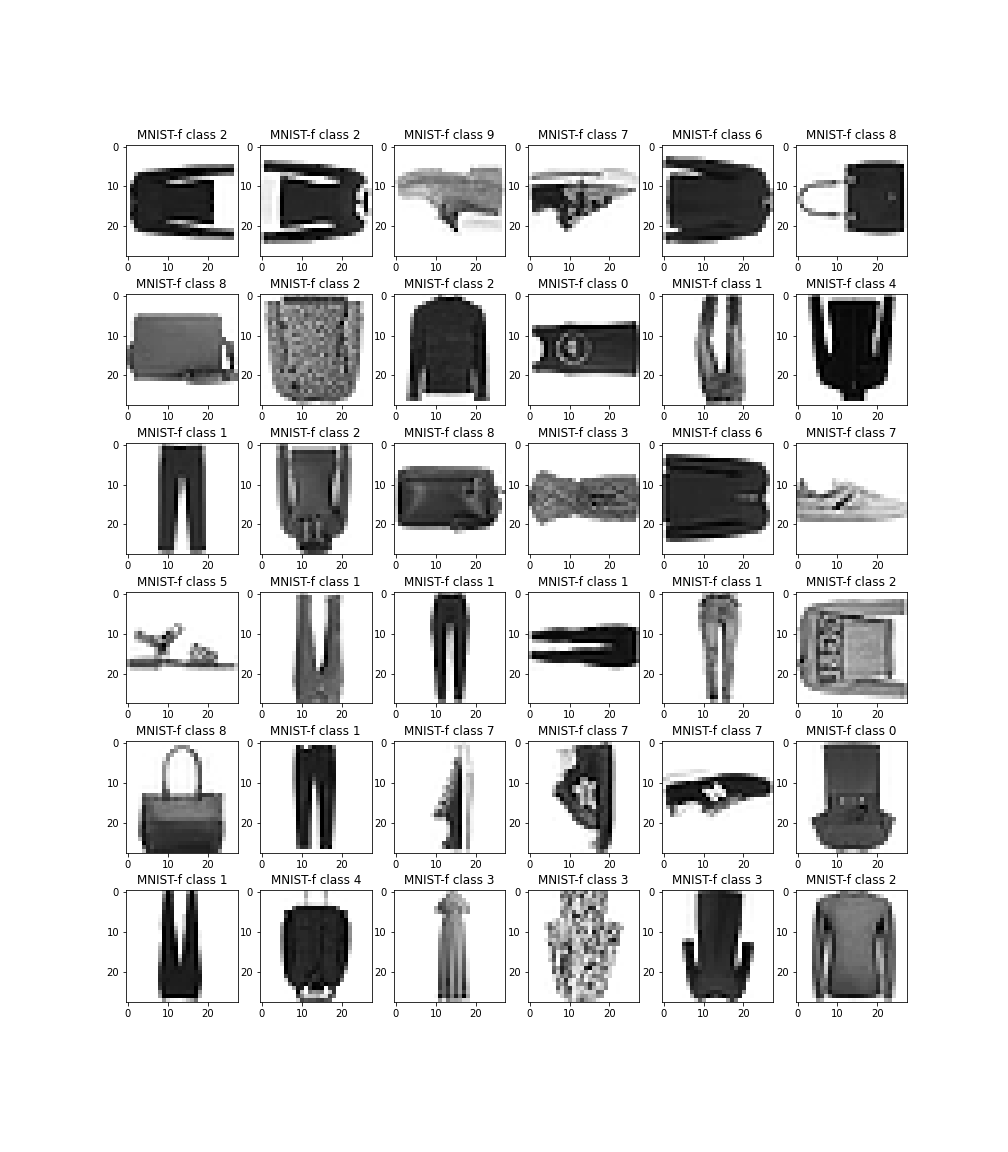
\includegraphics[width=\textwidth]{../notebooks/MNIST-f.png}
\caption{foo and bar.\label{fig:f}}
\end{figure}

\section{Benchmarks}

\section{}
\end{document}
